%-----------------------------------------------------------------------------%
% Document class
%-----------------------------------------------------------------------------%
\documentclass[a4paper,12pt,onecolumn,final]{article}
%-----------------------------------------------------------------------------%
% Geometry package for setting page margins
%-----------------------------------------------------------------------------%
\usepackage[paper=a4paper,vscale=0.8,hscale=0.85,centering]{geometry}
%-----------------------------------------------------------------------------%
% Helvet package for font
%-----------------------------------------------------------------------------%
\usepackage[scaled=0.92]{helvet}
\renewcommand{\familydefault}{\sfdefault}
%-----------------------------------------------------------------------------%
% Include special packages here
%-----------------------------------------------------------------------------%
\usepackage{amsmath,amsfonts,amssymb}
\usepackage{xcolor}
\usepackage{graphicx}
\usepackage{hyperref}
\usepackage{listings}
\lstset {backgroundcolor=\color{black!5}, basicstyle=\footnotesize, stringstyle=\color{red}, commentstyle=\color{green!50!black}, basicstyle=\footnotesize\ttfamily, keywordstyle=\color{blue}, 
}
%-----------------------------------------------------------------------------%


%-----------------------------------------------------------------------------%
\begin{document}
%-----------------------------------------------------------------------------%


%-----------------------------------------------------------------------------%
\noindent
\begin{tabular}{|p{0.2\textwidth}|p{0.75\textwidth}|}
\hline
\textbf{G14CAM} & \textbf{Computational Applied Mathematics}
\\
2017--2018 & \textcolor{red}{Coursework 1 Part D}
\\
\hline
\textbf{Name} & \textcolor{red}{Ella Taylor}
\\ 
\textbf{Student ID} & \textcolor{red}{4290562}
\\ 
\textbf{Date} & \today
\\
\hline
\textbf{Existing codes} & \textcolor{red}{Names of approved existing codes that you used}
\\
\hline
\end{tabular}
%-----------------------------------------------------------------------------%
% \textcolor{red}{LaTeX instruction: This TeX-file template can be compiled using PDFLaTeX.}
%-----------------------------------------------------------------------------%
\section*{Problem 1}

\subsection*{Problem 1.a}
\begin{lstlisting}[language=C++]
#include <iostream>
#include <cmath>
#include <cassert>
#include <iomanip>

void funct(double* f, double* y, double alpha, double beta)
{
f[0] = y[1];
f[1] = -pow(alpha,2)*sin(y[0])-pow(beta,2)*y[1];
}

void Forward_Euler(double* y, double h, int n_max, double alpha, double beta)
{

double f[2];
int i = 0;
double Energy;

std::cout<<std::setw(5)<<"tn"<<std::setw(15)<<"y1"<<std::setw(25)<<"y2"
<<std::setw(30)<<"Energy"<<std::endl;

while(i<=n_max)
    {

    Energy = 0.5*pow(y[1],2)+pow(alpha,2)*(1-cos(y[0]));

    std::cout<<std::setw(5)<<i*h<<std::setw(15)<<y[0]<<std::setw(25)<<y[1]
    <<std::setw(30)<<Energy<<std::endl;

    funct(f,y,alpha, beta);

    for (int j = 0; j<2; j++)
        {
        y[j] = y[j] + h*f[j];
        }
    i++;
    }
}

int main()
{
const double alpha = 1.0;
const double beta = 2.0;
const double pi = 3.14159265359;

double* y;
y = new double[2];
y[0] = pi/2.0;
y[1] = 0.0;

int n_max = 32;
//double T = 32;
double h = 0.25; //T/double(n_max); //= T/n_max

Forward_Euler(y, h, n_max, alpha,beta);

return 0;
}

\end{lstlisting}%

\subsection*{Problem 1.b}

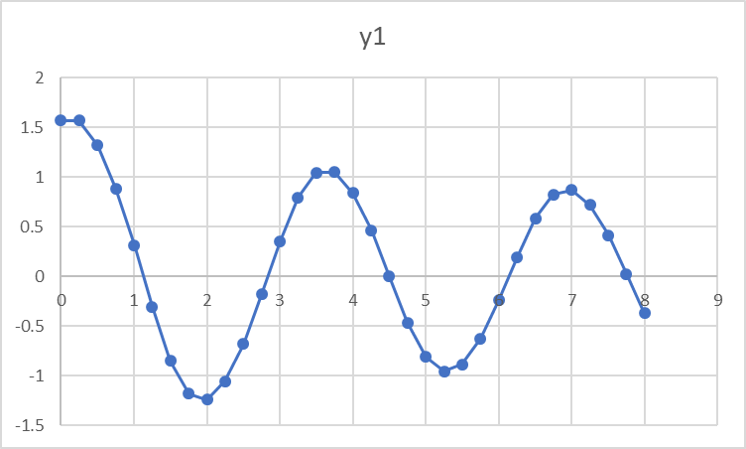
\includegraphics[scale=1]{CW_1D/CW_1DP1/Q1by1.png} 

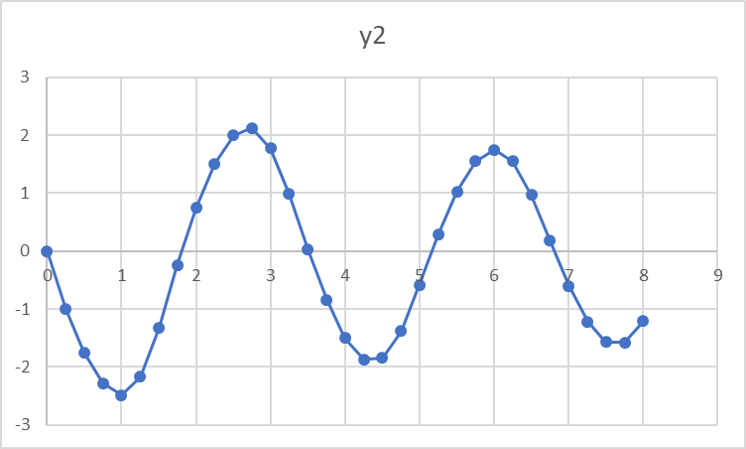
\includegraphics[scale=1]{CW_1D/CW_1DP1/Q1by2.png} 

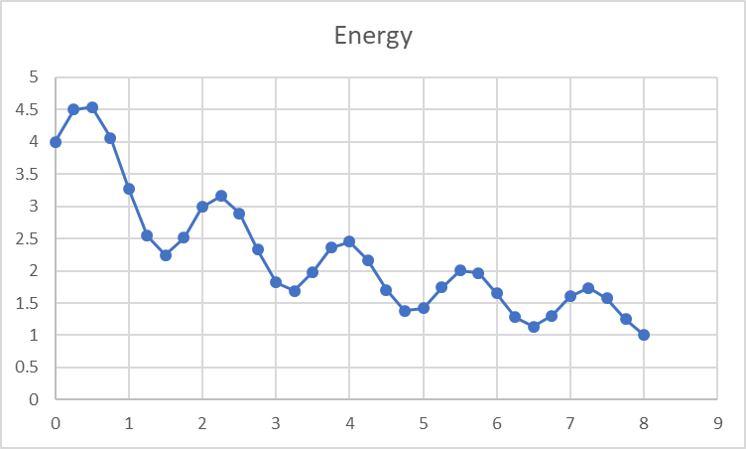
\includegraphics[scale=1]{CW_1D/CW_1DP1/Q1bEnergy.png} 

It is expected that energy will tend to zero as the system loses energy due to air resistance. The peaks and troughs in this graph correspond to the peaks and troughs in the above graphs.

\subsection*{Problem 1.c}

\begin{verbatim}


Testing different values of h and setting n_max to be very large, I found that
 for h less than or equal to the below values y1 converged to zero, otherwise
  they diverged. 

alpha = 1, beta = 2, theta_0 = pi/2 
Numerical upper bound for h = 0.55


alpha = 2, beta = 0.1, theta_0 = pi/2
Numerical upper bound for h = 0.0034

\end{verbatim}

%-----------------------------------------------------------------------------%
\section*{Problem 2}
\subsection*{Problem 2.a}
\subsection*{Problem 2.b}
\begin{lstlisting}[language=C++]
#include <iostream>
#include <cmath>
#include <iomanip>

void funct(double* f, double* y, double alpha, double beta)
{
f[0] = y[1];
f[1] = -pow(alpha,2)*sin(y[0])-pow(beta,2)*y[1];
}

void Newton_Method(double TOL, double* y_1, double* y_2, int n_max, 
double alpha, double beta, double h)
{
double* u;
u = new double[2];

int counter = 0;

double *f;
f = new double[2];
double F[2];

double F_norm = 10.0;
double determinant;
double Energy;

std::cout<< "n"<<std::setw(12)<<"y1"<<std::setw(18)<<"y2"<<std::setw(25)<<"F_norm"
<<std::setw(32)<<"Energy"<<std::endl;

for (int i = 1; i <= n_max; i++)
    {
    //Setting initial guess y_n+1(0) = y_n

   std::cout<<std::endl<<i;

    y_1[i] = y_1[i-1];
    y_2[i] = y_2[i-1];

    // calculating initial norm
     u[0] = y_1[i];
     u[1] = y_2[i];
     funct(f,u,alpha,beta);

    F[0] = y_1[i] - y_1[i-1] - h*f[0];
    F[1] = y_2[i] - y_2[i-1] - h*f[1];
    F_norm = sqrt(pow(F[0],2) + pow(F[1],2));

    while (F_norm >= TOL)
        {
        F_norm = 0;

        //std::cout<<std::setw(7)<<counter;
        counter++;

        // update y1 and y2
        u[0] = y_1[i];
        u[1] = y_2[i];
        funct(f,u,alpha,beta);
        determinant = (1.0 + pow(h,2)*pow(alpha,2)*cos(y_1[i]));

        y_1[i] +=  (-1.0/determinant) * (F[0] + h*F[1]);
       //std::cout<<std::setw(12)<<y_1[i];
        y_2[i] += (-1.0/determinant) * ( (-h*pow(alpha,2)*cos(y_1[i])*F[0]) + F[1]);
        //std::cout<<std::setw(18)<<y_2[i];

        // calculate norm for updated y and y2 values
        u[0] = y_1[i];
        u[1] = y_2[i];
        funct(f,u,alpha,beta);
        F[0] = y_1[i] - y_1[i-1] - h*f[0];
        F[1] = y_2[i] - y_2[i-1] - h*f[1];
        F_norm = sqrt(pow(F[0],2) + pow(F[1],2));

        //std::cout<<std::setw(25)<<F_norm<<std::endl;
        }
        counter=0;

        Energy = 0.5*pow(y_2[i],2)+pow(alpha,2)*(1-cos(y_1[i]));
       // std::cout<<"Energy = "<<Energy<<std::endl;

       std::cout<<std::setw(14)<<y_1[i];
       std::cout<<std::setw(18)<<y_2[i];
       std::cout<<std::setw(25)<<F_norm;
       std::cout<<std::setw(32)<<Energy<<std::endl;

    }
delete[] f;
delete[] u;
}

int main()
{
double alpha = 2.0;
double beta = 0.0;
double pi = 3.14159265359;

//double T = 8.0;
int n_max = 32;
double h = T/(double)(n_max);

double* y_1;
double* y_2;

y_1 = new double[n_max+1];
y_2 = new double[n_max+1];


y_1[0] = pi/2.0;
y_2[0] = 0.0;

for (int i = 1; i<n_max; i++)
{
    y_1[i] = 0;
    y_2[i] = 0;
}

double TOL = pow(10,-12);

//From backward Euler have F(y_n+1) = y_n+1 - y_n -hf(y_n+1,t+1) = 0
//Then apply Newtons method to this

Newton_Method(TOL, y_1, y_2, n_max, alpha, beta, h);



delete[] y_1;
delete[] y_2;

return 0;
}

\end{lstlisting}%
\subsection*{Problem 2.c}

\includegraphics[scale=1]{../../cw1d2c.png} 

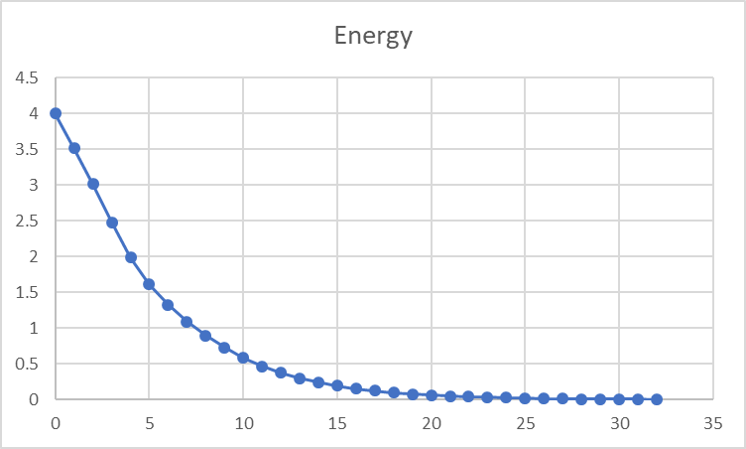
\includegraphics[scale=1]{CW_1D/CW1_DP2/Q2cEnergy(2).png} 

\begin{verbatim}
As beta = 0 = sqrt(c/m), c = 0. So there is no air resistance. This is not the
 case in the true physics of the problem.
\end{verbatim}

\subsection*{Problem 2.d}

\begin{verbatim}

Does not converge to zero for all h. If h is too large then Newton's method
 converges to another root or diverges to infinity.
Numerically found upper bound for h = 0.9201

\end{verbatim}


%-----------------------------------------------------------------------------%
\end{document}
%-----------------------------------------------------------------------------%
